\documentclass[11pt,oneside]{article}	%use"amsart"insteadof"article"forAMSLaTeXformat
\usepackage{geometry}		%Seegeometry.pdftolearnthelayoutoptions.Therearelots.
\geometry{letterpaper}		%...ora4paperora5paperor...
%\geometry{landscape}		%Activateforforrotatedpagegeometry
%\usepackage[parfill]{parskip}		%Activatetobeginparagraphswithanemptylineratherthananindent
\usepackage{graphicx}				%Usepdf,png,jpg,orepsßwithpdflatex;useepsinDVImode
								%TeXwillautomaticallyconverteps-->pdfinpdflatex		
\usepackage{amssymb}
\usepackage{hyperref}

%----macros begin---------------------------------------------------------------
\usepackage{color}
\usepackage{amsthm}

\def\conv{\mbox{\textrm{conv}\,}}
\def\aff{\mbox{\textrm{aff}\,}}
\def\E{\mathbb{E}}
\def\R{\mathbb{R}}
\def\Z{\mathbb{Z}}
\def\tex{\TeX}
\def\latex{\LaTeX}
\def\v#1{{\bf #1}}
\def\p#1{{\bf #1}}
\def\T#1{{\bf #1}}

\def\vet#1{{\left(\begin{array}{cccccccccccccccccccc}#1\end{array}\right)}}
\def\mat#1{{\left(\begin{array}{cccccccccccccccccccc}#1\end{array}\right)}}

\def\lin{\mbox{\rm lin}\,}
\def\aff{\mbox{\rm aff}\,}
\def\pos{\mbox{\rm pos}\,}
\def\cone{\mbox{\rm cone}\,}
\def\conv{\mbox{\rm conv}\,}
\newcommand{\homog}[0]{\mbox{\rm homog}\,}
\newcommand{\relint}[0]{\mbox{\rm relint}\,}

%----macros end-----------------------------------------------------------------

\title{Modeling Geometry with Assemblies in SysML
\footnote{This document is part of the \emph{Linear Algebraic Representation with CoChains} (LAR-CC) framework~\cite{cclar-proj:2013:00}. \today}
}
%\author{TheAuthor}
%\date{}							%Activatetodisplayagivendateornodate

\begin{document}
\maketitle
\nonstopmode

\begin{abstract}
In this module a preliminary concept implementation is provided for the possible introduction of a novel kind of 3D diagram in SysML. Such ``Assembly" Diagram in used to specify an operable description of the 3D geometry of a system part.
\end{abstract}

\tableofcontents

%===============================================================================
\section{Introduction}
%===============================================================================
%-------------------------------------------------------------------------------
\subsection{bbbbbbbb}
%-------------------------------------------------------------------------------
%===============================================================================
\section{Implementation}
%===============================================================================
%-------------------------------------------------------------------------------
\subsection{Diagram initialization}
%-------------------------------------------------------------------------------

\paragraph{Uniform cell sizing}

A cuboidal 3-complex is generated by the script below, where the cells have uniform dimension on each coordinate direction. 

%-------------------------------------------------------------------------------
@D Diagram initialization
@{""" Diagram initialization """
def assemblyDiagramInit(shape):
	print "\n shape =",shape
	# shape must be 3D, i.e. a python array with 3 indices
	assert len(shape) == 3
	diagram = larCuboids(shape)
	return diagram
@}
%-------------------------------------------------------------------------------

\paragraph{Non-uniform cell sizing}

The parameter \texttt{quoteList} is used here to generate the new vertices of the \texttt{diagram}, previously generated with uniform spacing between the cell vertices in every coordinate direction.
Each \texttt{pattern} in \texttt{quoteList} is a list of positive numbers, each corresponding to the size of the corresponding "coordinate stripe".

%-------------------------------------------------------------------------------
@D Diagram initialization (non-uniform sizing)
@{""" Diagram initialization """
def assemblyDiagramInit (shape):
	def assemblyDiagram (quoteList):
		print "\n shape =",shape
		# shape and quoteList must be 3D, i.e. a python array with 3 indices
		assert (len(shape) == 3) and (len(quoteList) == 3)
		coordList = [list(cumsum([0]+pattern)) for pattern in quoteList]
		verts = CART(coordList)
		_,CV = larCuboids(shape)
		return verts,CV
	return assemblyDiagram
@}
%-------------------------------------------------------------------------------


\paragraph{Diagram scaling to cuboid of given size}
The \texttt{size} parameter is the array of lateral dimensions to which to scale the 
\texttt{diagram} parameter. \texttt{size} must be an array of 3 numbers; \texttt{diagram} is
a LAR model

%-------------------------------------------------------------------------------
@D Diagram scaling to sized cuboid
@{""" Diagram scaling to given size """
def unitDiagram(diagram, size=[1,1,1]):
	V,CV = diagram
	print "\n shape =",shape
	# size must be a python array with 3 numbers
	assert (len(size) == 3) and (AND(AA(ISNUM)(size)) == True)
	V_ = array(V) / AA(float)(max(V))
	V = (V_ * size).tolist()
	diagram = V,CV
	return diagram
@}
%-------------------------------------------------------------------------------



%-------------------------------------------------------------------------------
\subsection{Cell numbering}
%-------------------------------------------------------------------------------


\paragraph{Drawing numbers of cells}

%-------------------------------------------------------------------------------
@D Drawing numbers of cells
@{""" Drawing numbers of cells """
def cellNumbering (larModel,hpcModel):
	V,CV = larModel
	def cellNumbering0 (cellSubset,color=WHITE,scalingFactor=1):
		text = TEXTWITHATTRIBUTES (TEXTALIGNMENT='centre', TEXTANGLE=0, 
							TEXTWIDTH=0.1*scalingFactor, 
							TEXTHEIGHT=0.2*scalingFactor, 
							TEXTSPACING=0.025*scalingFactor)
		hpcList = [hpcModel]
		for cell in cellSubset:
			point = CCOMB([V[v] for v in CV[cell]])
			hpcList.append(T([1,2,3])(point)(COLOR(color)(text(str(cell)))))
		return STRUCT(hpcList)
	return cellNumbering0
@}
%-------------------------------------------------------------------------------


%-------------------------------------------------------------------------------
\subsection{Diagram segmentation}
%-------------------------------------------------------------------------------

\paragraph{Boundary cells ($3D\to 2D$) computation}
The computations of boundary cells is executed by calling the \texttt{boundaryCells} from the \texttt{larcc} module.

%-------------------------------------------------------------------------------
@D Boundary cells ($3D\to 2D$) computation
@{def lar2boundaryFaces(CV,FV):
	""" Boundary cells computation """
	return boundaryCells(CV,FV)
@}
%-------------------------------------------------------------------------------

\paragraph{Interior partitions ($3D\to 2D$) computation}
The indices of the boundary 2-cells are returned in \texttt{boundarychain2D}, and subtracted from the set $\{0,1,\ldots,|E|-1\}$ in order to return the indices of the \texttt{interiorCells}.
%-------------------------------------------------------------------------------
@D Interior partitions ($3D\to 2D$) computation
@{def lar2InteriorFaces(CV,FV):
	""" Boundary cells computation """
	boundarychain2D = boundaryCells(CV,FV)
	totalChain2D = range(len(FV))
	interiorCells = set(totalChain2D).difference(boundarychain2D)
	return interiorCells
@}
%-------------------------------------------------------------------------------


%-------------------------------------------------------------------------------
\subsection{Subdiagram mapping}
%-------------------------------------------------------------------------------

The aim of this section is to allow for separate development of subdiagrams of a geometric diagram.
When satisfied with the current design situation,  the developer may map a whole diagram into a single 3D cell of the upper-level diagram --- in the following called the \emph{master} diagram.
Of course, such nesting may happen several times within a (father) master, producing a hierarchical decomposition (of any depth) of the geometry diagrams.


\paragraph{Task decomposition}
The procedure to map a diagram to a sub diagram is described below in a top-down manner,
decomposing the task into an ordered set of subtasks.
%-------------------------------------------------------------------------------
@D Subdiagram to diagram mapping
@{
@< 3D window to viewport transformation @>

def diagram2cell(diagram,master,cell):
	mat = diagram2cellMatrix(diagram)(master,cell)
	diagram =larApply(mat)(diagram)	
	
	"""
	# yet to finish coding
	V, CV1, CV2, n12 = vertexSieve(master,diagram)
	masterBoundaryFaces = boundaryOfChain(CV,FV)([cell])
	diagramBoundaryFaces = lar2boundaryFaces(CV,FV)
	"""
	V = master[0] + diagram[0]
	offset = len(master[0])
	CV = [c for k,c in enumerate(master[1]) if k != cell] + [[v+offset for v in c] for c in diagram[1]]
	master = V, CV
	return master
@}
%-------------------------------------------------------------------------------

\paragraph{3D window to viewport transformation}
%-------------------------------------------------------------------------------
@D 3D window to viewport transformation
@{""" 3D window to viewport transformation """
def diagram2cellMatrix(diagram):
	def diagramToCellMatrix0(master,cell):
		wdw = min(diagram[0]) + max(diagram[0])			# window3D
		cV = [master[0][v] for v in master[1][cell]]
		vpt = min(cV) + max(cV)								# viewport3D
		print "\n window3D =",wdw
		print "\n viewport3D =",vpt
		
		mat = zeros((4,4))
		mat[0,0] = (vpt[3]-vpt[0])/(wdw[3]-wdw[0])
		mat[0,3] = vpt[0] - mat[0,0]*wdw[0]
		mat[1,1] = (vpt[4]-vpt[1])/(wdw[4]-wdw[1])
		mat[1,3] = vpt[1] - mat[1,1]*wdw[1]
		mat[2,2] = (vpt[5]-vpt[2])/(wdw[5]-wdw[2])
		mat[2,3] = vpt[2] - mat[2,2]*wdw[2]
		mat[3,3] = 1
		print "\n mat =",mat
		return mat
	return diagramToCellMatrix0
@}
%-------------------------------------------------------------------------------


%===============================================================================
\section{Library export}
%===============================================================================
%-------------------------------------------------------------------------------
\subsection{Exporting the library}
%-------------------------------------------------------------------------------

%-------------------------------------------------------------------------------
@O lib/py/sysml.py
@{@< Initial import of modules @>
@< To compute the boundary (d-1)-chain of a given d-chain @>
@< Diagram initialization (non-uniform sizing) @>
@< Boundary cells ($3D\to 2D$) computation @>
@< Interior partitions ($3D\to 2D$) computation @>
@< Diagram scaling to sized cuboid @>
from myfont import *
@< Drawing numbers of cells @>
@< Subdiagram to diagram mapping @>
@}
%-------------------------------------------------------------------------------

%===============================================================================
\section{Tests}
%===============================================================================
%-------------------------------------------------------------------------------
\subsection{Diagram initialization}
%-------------------------------------------------------------------------------

%-------------------------------------------------------------------------------
@O test/py/sysml/test01.py
@{""" testing initial steps of Assembly Diagram construction """
@< Initial import of modules @>
from sysml import *

shape = [1,2,2]
sizePatterns = [[1],[2,1],[0.8,0.2]]
diagram = assemblyDiagramInit(shape)(sizePatterns)
print "\n diagram =",diagram
VIEW(SKEL_1(STRUCT(MKPOLS(diagram))))

VV,EV,FV,CV = gridSkeletons(shape)
boundaryFaces = lar2boundaryFaces(CV,FV)
interiorFaces = list(set(range(len(FV))).difference(boundaryFaces))
print "\n boundary faces =",boundaryFaces
print "\n interior faces =",interiorFaces
diagram1 = unitDiagram(diagram)
VIEW(SKEL_1(STRUCT(MKPOLS(diagram1))))

hpc = SKEL_1(STRUCT(MKPOLS(diagram1)))
V = diagram1[0]
hpc = cellNumbering ((V,FV),hpc)(interiorFaces,YELLOW,.5)
VIEW(hpc)
hpc = cellNumbering ((V,EV),hpc)([for f in interiorFaces],GREEN,.4)
VIEW(hpc)
hpc = cellNumbering ((V,VV),hpc)(range(len(VV)),RED,.3)
VIEW(hpc)

@}
%-------------------------------------------------------------------------------

%-------------------------------------------------------------------------------
\subsection{Diagram merging}
%-------------------------------------------------------------------------------

%-------------------------------------------------------------------------------
@O test/py/sysml/test02.py
@{""" definition and merging of two diagrams into a single diagram """
@< Initial import of modules @>
from sysml import *

master = assemblyDiagramInit([2,2,2])([[.4,.6],[.4,.6],[.4,.6]])
diagram = assemblyDiagramInit([3,3,3])([[.4,.2,.4],[.4,.2,.4],[.4,.2,.4]])
VIEW(SKEL_1(STRUCT([DRAW(master),T(2)(1),DRAW(diagram)])))

hpc = SKEL_1(STRUCT(MKPOLS(master)))
hpc = cellNumbering (master,hpc)(range(len(master[1])),WHITE,.5)
VIEW(hpc)

master = diagram2cell(diagram,master,7)
VIEW(SKEL_1(STRUCT( MKPOLS(master) )))

@}
%-------------------------------------------------------------------------------

%-------------------------------------------------------------------------------
\subsection{Diagram visualization}
%-------------------------------------------------------------------------------


%-------------------------------------------------------------------------------
@O test/py/sysml/test03.py
@{""" definition and merging of two diagrams into a single diagram """
@< Initial import of modules @>
from sysml import *

master = assemblyDiagramInit([2,2,2])([[.4,.6],[.4,.6],[.4,.6]])
diagram = assemblyDiagramInit([3,3,3])([[.4,.2,.4],[.4,.2,.4],[.4,.2,.4]])

VV,EV,FV,CV = gridSkeletons([2,2,2])
V,CV = master
hpc = SKEL_1(STRUCT(MKPOLS(master)))
hpc = cellNumbering (master,hpc)(range(len(CV)),CYAN,.5)
VIEW(hpc)

master = diagram2cell(diagram,master,7)
VIEW(SKEL_1(STRUCT( MKPOLS(master) )))

VIEW(EXPLODE(1.5,1.5,1.5)(MKPOLS(larFacets(master))))

masterBoundaryFaces = boundaryOfChain(CV,FV)([7])
diagramBoundaryFaces = lar2boundaryFaces(CV,FV)
@}
%-------------------------------------------------------------------------------

\begin{figure}[htbp] %  figure placement: here, top, bottom, or page
   \centering
   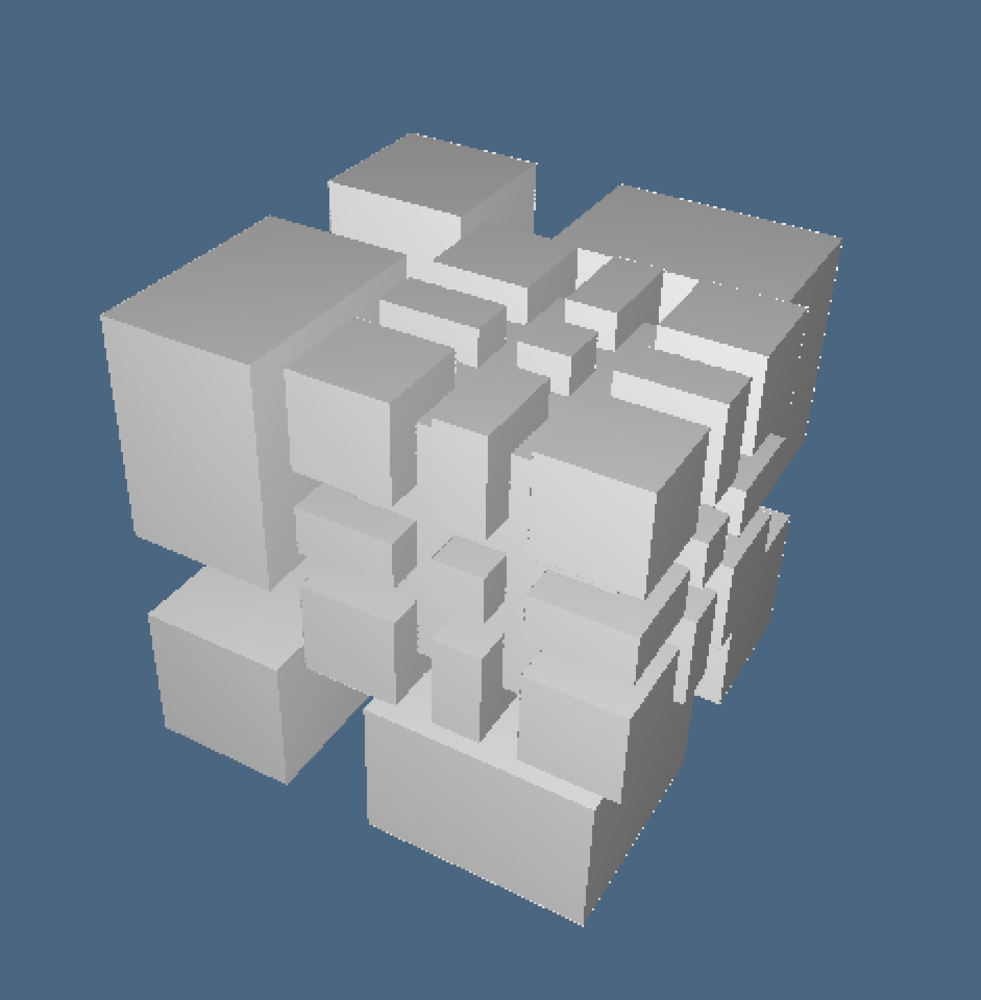
\includegraphics[height=0.49\linewidth,width=0.49\linewidth]{images/mastermerged} 
   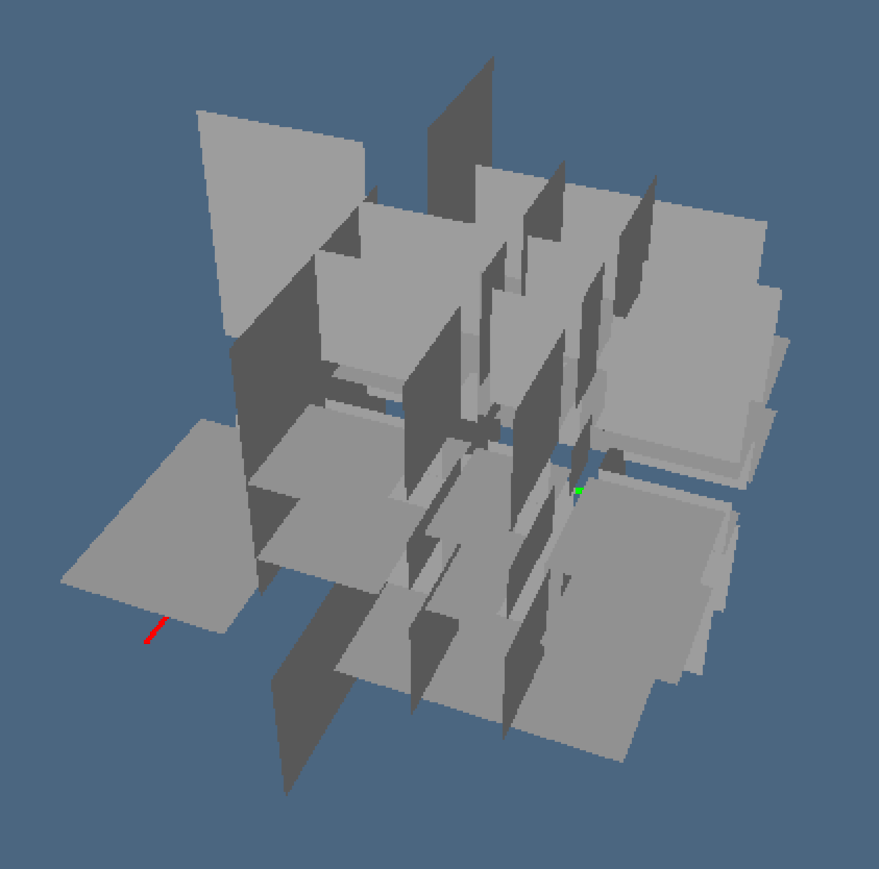
\includegraphics[height=0.49\linewidth,width=0.49\linewidth]{images/masterfacets} 
   \caption{Example of a geometry diagram merged in a master diagram}
   \label{fig:mastermerged}
\end{figure}


\paragraph{progressive refinement of a block diagram}

%-------------------------------------------------------------------------------
@O test/py/sysml/test04.py
@{""" progressive refinement of a block diagram """
@< Initial import of modules @>
from sysml import *
DRAW = COMP([VIEW,STRUCT,MKPOLS])

master = assemblyDiagramInit([5,5,2])([[.3,3.2,.1,5,.3],[.3,4,.1,2.9,.3],[.3,2.7]])
V,CV = master
hpc = SKEL_1(STRUCT(MKPOLS(master)))
hpc = cellNumbering (master,hpc)(range(len(CV)),CYAN,2)
VIEW(hpc)

toRemove = [13,33,17,37]
master = V,[cell for k,cell in enumerate(CV) if not (k in toRemove)]
DRAW(master)

hpc = SKEL_1(STRUCT(MKPOLS(master)))
hpc = cellNumbering (master,hpc)(range(len(master[1])),CYAN,2)
VIEW(hpc)

toMerge = 29
cell = MKPOL([master[0],[[v+1 for v in  master[1][toMerge]]],None])
VIEW(STRUCT([hpc,cell]))

diagram = assemblyDiagramInit([3,1,2])([[2,1,2],[.3],[2.2,.5]])
master = diagram2cell(diagram,master,toMerge)
hpc = SKEL_1(STRUCT(MKPOLS(master)))
hpc = cellNumbering (master,hpc)(range(len(master[1])),CYAN,2)
VIEW(hpc)

toRemove = [47]
master = master[0], [cell for k,cell in enumerate(master[1]) if not (k in toRemove)]
DRAW(master)

hpc = SKEL_1(STRUCT(MKPOLS(master)))
hpc = cellNumbering (master,hpc)(range(len(master[1])),CYAN,2)
VIEW(hpc)

toMerge = 34
cell = MKPOL([master[0],[[v+1 for v in  master[1][toMerge]]],None])
VIEW(STRUCT([hpc,cell]))

diagram = assemblyDiagramInit([5,1,3])([[1.5,0.9,.2,.9,1.5],[.3],[1,1.4,.3]])
master = diagram2cell(diagram,master,toMerge)
hpc = SKEL_1(STRUCT(MKPOLS(master)))
hpc = cellNumbering (master,hpc)(range(len(master[1])),CYAN,2)
VIEW(hpc)

toRemove = [53,59]
master = master[0], [cell for k,cell in enumerate(master[1]) if not (k in toRemove)]
DRAW(master)
@}
%-------------------------------------------------------------------------------


%===============================================================================
\appendix
\section{Utilities}
%===============================================================================

%-------------------------------------------------------------------------------
@D To compute the boundary (d-1)-chain of a given d-chain
@{
def boundaryOfChain(cells,facets):
	csrBoundaryMat = boundary(cells,facets)
	csrChain = zeros((len(cells),1))
	def boundaryOfChain0(chain):
		for cell in chain:  csrChain[cell,0]=1.0
		csrBoundaryChain = matrixProduct(csrBoundaryMat, csrChain)
		boundaryCells = [k for k,val in enumerate(csrBoundaryChain.tolist()) 
							if val == [1.0]]
		return boundaryCells
	return boundaryOfChain0
@}
%-------------------------------------------------------------------------------


%-------------------------------------------------------------------------------
\subsection{Initial import of modules}
%-------------------------------------------------------------------------------

\paragraph{Initial import of modules}

%-------------------------------------------------------------------------------
@D Initial import of modules
@{from pyplasm import *
from scipy import *
import os,sys
""" import modules from larcc/lib """
sys.path.insert(0, 'lib/py/')
from lar2psm import *
from simplexn import *
from larcc import *
from largrid import *
from mapper import *
from boolean import *
@}
%-------------------------------------------------------------------------------

\bibliographystyle{amsalpha}
\bibliography{sysml}

\end{document}
